\begin{frame}[fragile]{Inicios IA}
	\vspace{10px}
	\pause
	\metroset{block=fill}
	\begin{block}{Laboratorios de IA}
		\begin{itemize}
			\item SRI: Shakey, A*, ARPANET.
			\pause
			\item Laboratorio de IA del MIT: McCarthy (Lisp) y Stallman.
			\pause
			\item Robotics Institute: Sandstorm y Highlander.
		\end{itemize}
	\end{block}
	\begin{figure}
		\centering
		\pause
		\begin{subfigure}{0.33\textwidth}
			\centering
			\includegraphics[scale=0.038]{./EtapaModerna/Imagenes/sri.jpg}
			\caption{SRI \href{https://es.m.wikipedia.org/wiki/Archivo:SRI_International_HQ.jpg}{Wikidata}}
		\end{subfigure}
		\pause
		\begin{subfigure}{0.32\textwidth}
			\centering
			\includegraphics[scale=0.04]{./EtapaModerna/Imagenes/mit_ai.jpg}
			\caption{MIT AI Lab \href{https://commons.wikimedia.org/wiki/File:Stata_Center1.jpg}{Wikidata}}
		\end{subfigure}
		\pause
		\begin{subfigure}{0.33\textwidth}
			\centering
			\includegraphics[scale=0.026]{./EtapaModerna/Imagenes/robotics_institute.jpg}
			\caption{Robotics Institute \href{https://commons.wikimedia.org/wiki/File:National_Robotics_Engineering_Center.JPG}{Wikidata}}
		\end{subfigure}
	\end{figure}
\end{frame}

\begin{frame}[fragile]{Brazos Robóticos}
\vspace{10px}
\pause
\metroset{block=fill}
\begin{block}{Brazos Robóticos}
	\begin{itemize}
		\item Stanford Arm: eléctrico con 6 grados de libertad.
		\pause
		\item PUMA: programable fabricado por General Motors.
		\pause
		\item SCARA: primer brazo con giro en el eje Z.
	\end{itemize}
\end{block}
\begin{figure}
	\centering
	\pause
	\begin{subfigure}{0.33\textwidth}
		\centering
		\includegraphics[scale=0.08]{./EtapaModerna/Imagenes/stanford_arm.jpg}
		\caption{Stanford Arm \href{https://www.flickr.com/photos/gildardo/6186967797}{Flickr}}
	\end{subfigure}
	\pause
	\begin{subfigure}{0.32\textwidth}
		\centering
		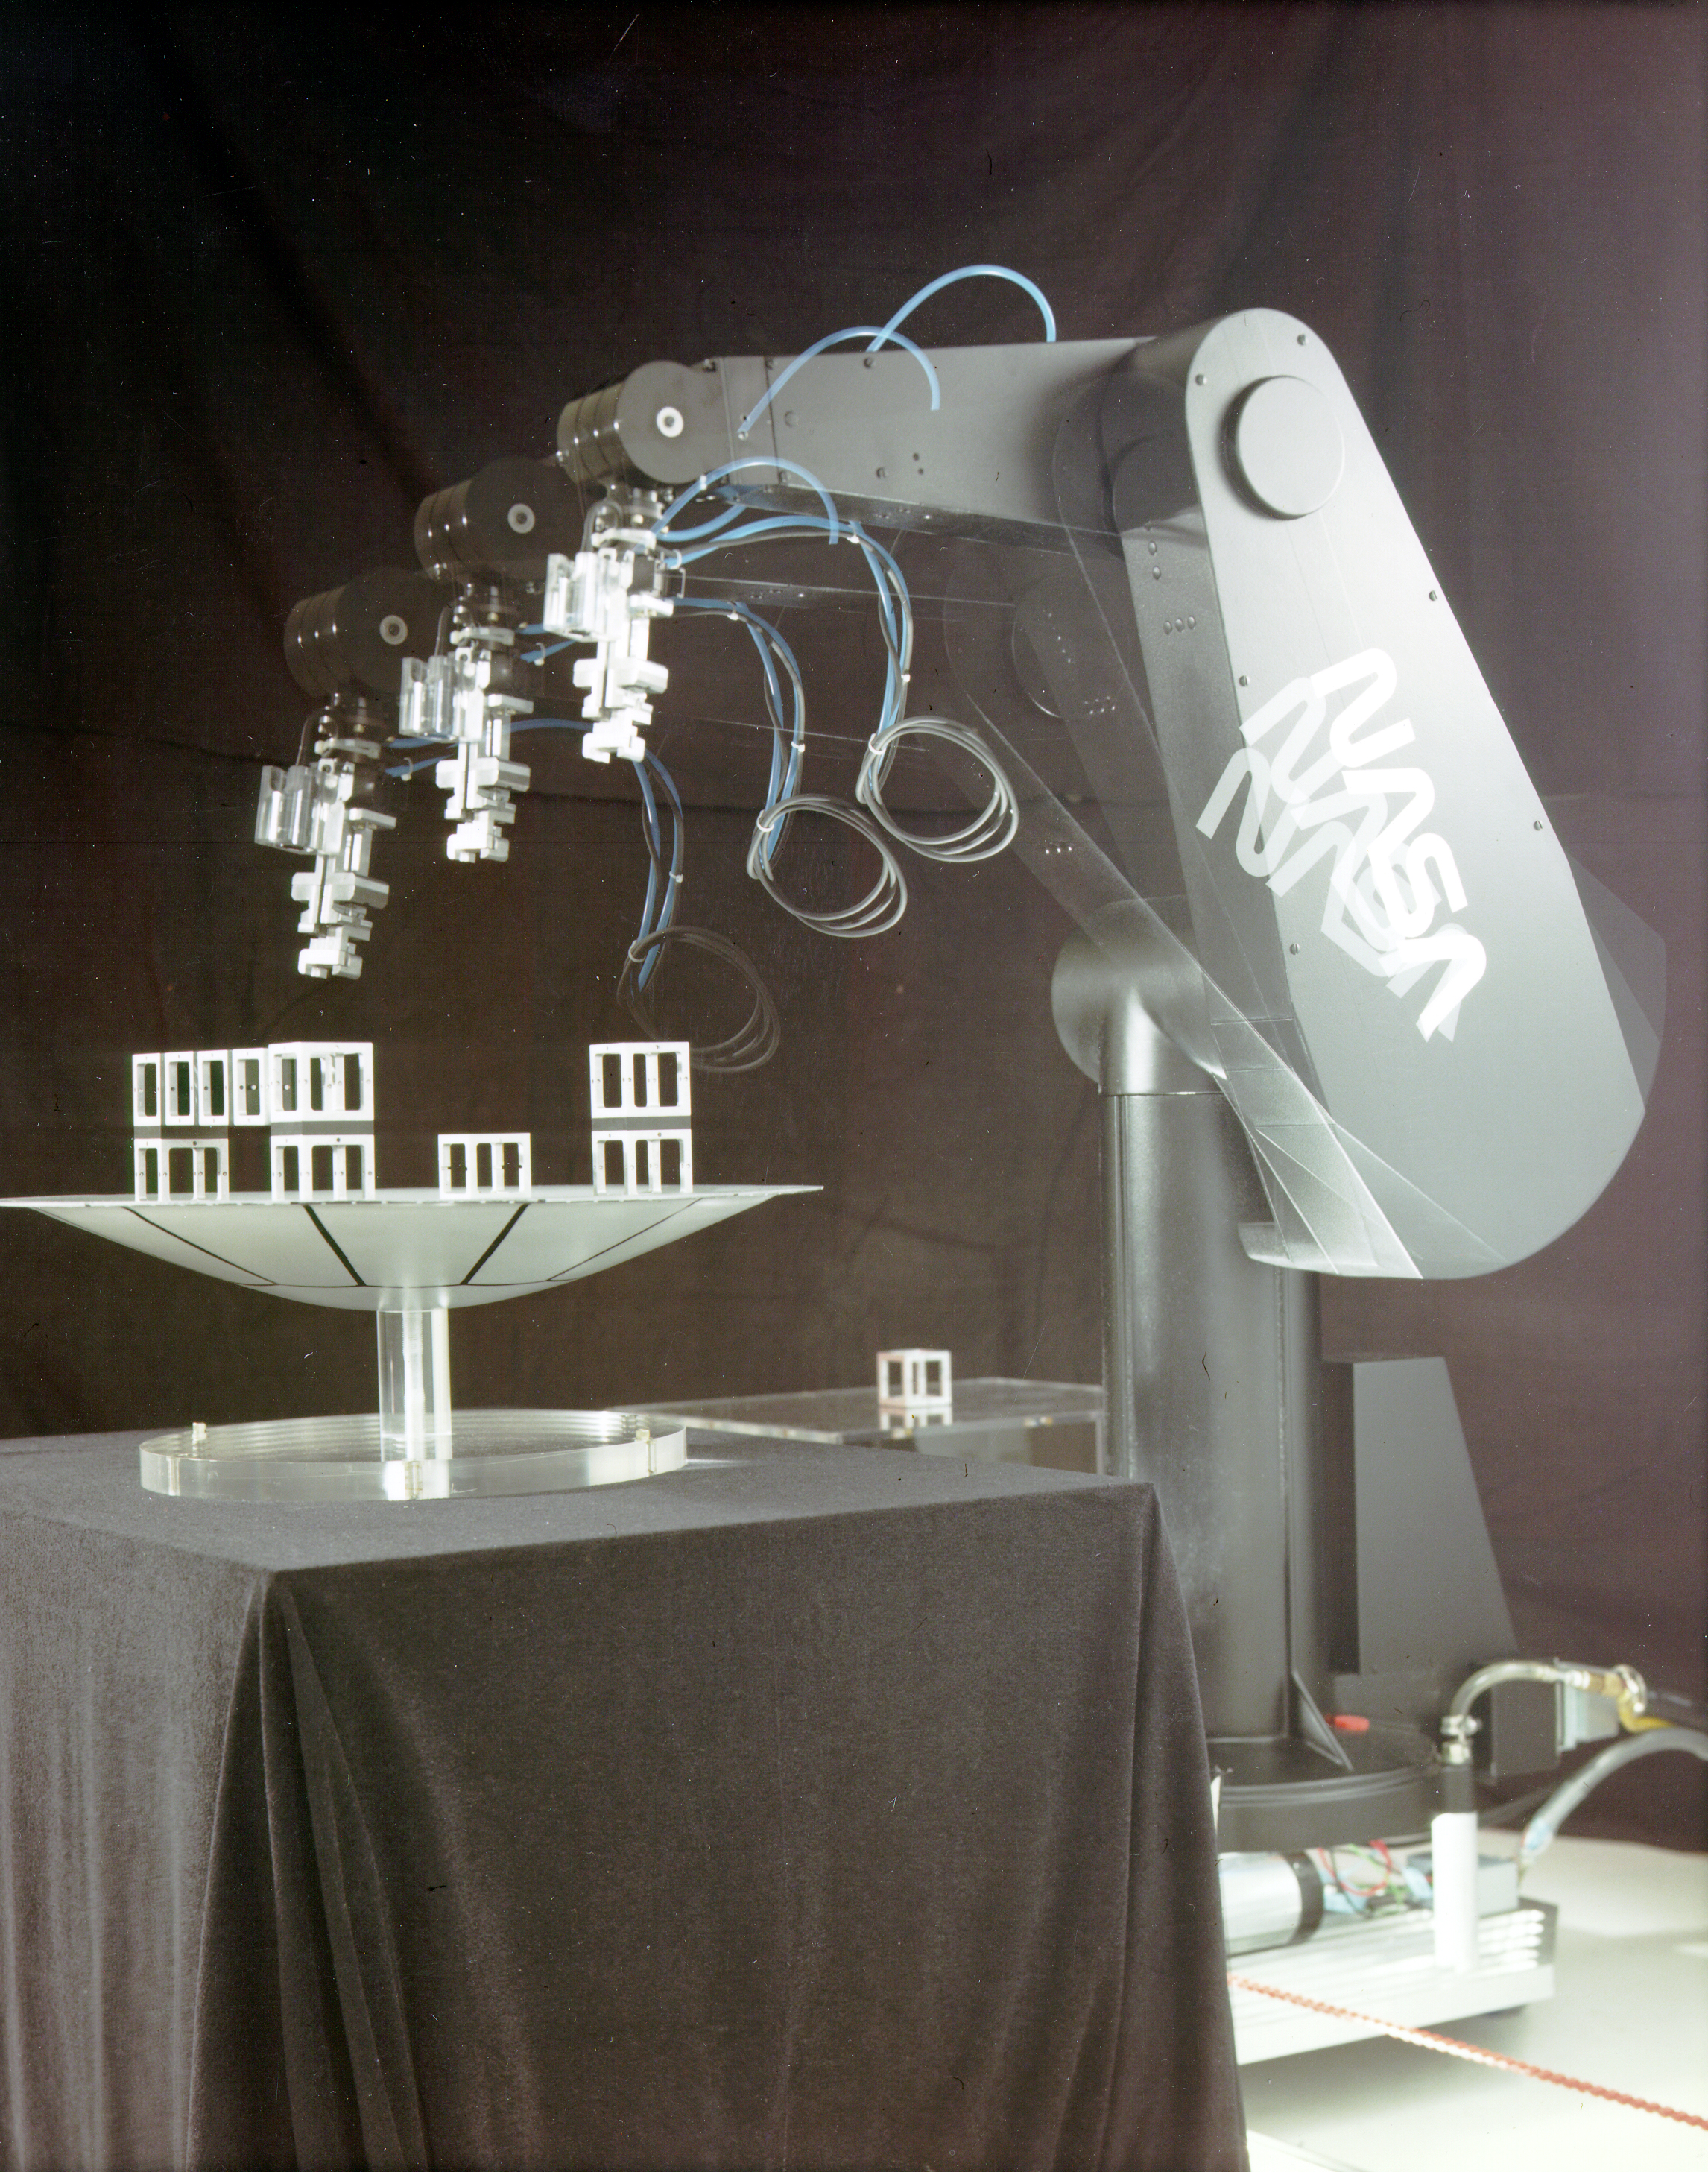
\includegraphics[scale=0.12]{./EtapaModerna/Imagenes/puma.jpg}
		\caption{PUMA \href{https://es.m.wikipedia.org/wiki/Archivo:Puma_Robotic_Arm_-_GPN-2000-001817.jpg}{Wikidata}}
	\end{subfigure}
	\pause
	\begin{subfigure}{0.33\textwidth}
		\centering
		\includegraphics[scale=0.3]{./EtapaModerna/Imagenes/SCARA.jpg}
		\caption{SCARA \href{https://commons.wikimedia.org/wiki/File:KUKA_Industrial_Robot_KR10_SCARA.jpg}{Wikidata}}
	\end{subfigure}
\end{figure}
\end{frame}

\begin{frame}[fragile]{Movimiento}
\vspace{10px}
\pause
\metroset{block=fill}
\begin{block}{Avance en el movimiento}
	\begin{itemize}
		\item Antecesores: RB5X, Phony Pony, WAP, Aquarobot, ...
		\pause
		\item ASIMO: \href{https://www.youtube.com/watch?v=mI58DU1hu14}{Vídeo}
	\end{itemize}
\end{block}
\begin{figure}
	\centering
	\pause
	\includegraphics[scale=0.12]{./EtapaModerna/Imagenes/asimo.jpg}
	\caption{ASIMO \href{https://es.m.wikipedia.org/wiki/Archivo:ASIMO_4.28.11.jpg}{Wikidata}}
\end{figure}
\end{frame}